\section{Workflow}
Preamble: I expand on the stages I have seen, not on those I have not seen.
I am part of this project; I mention what I have done \dots

\begin{figure}[ht]
    \centering
    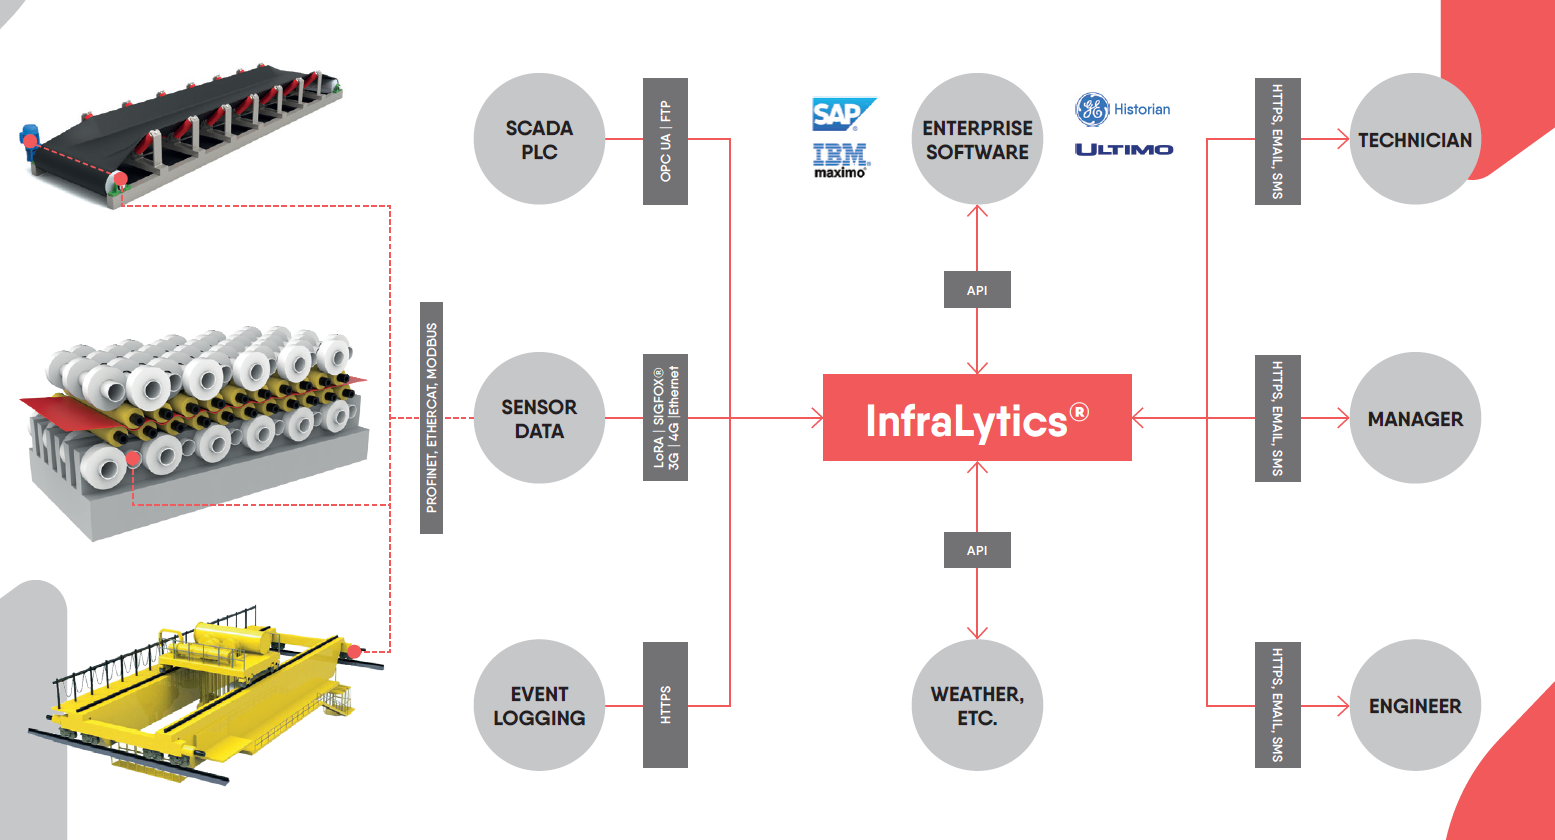
\includegraphics[width=\textwidth]{how_it_works_plan_owner.png}
    \caption{\acl{SaaS} Workflow (Source:~\cite{Misc:zensor_official_website})}
    \label{fig:zensor_flow}
\end{figure}

\subsubsection{Structure of a Deployable Script}\label{subsection:script_structure}
\[\begin{tikzcd}
		&& Datasource \\
		&& {} \\
		Load && Process && Write
		\arrow[from=3-1, to=3-3]
		\arrow[from=3-3, to=3-5]
		\arrow[from=1-3, to=3-1]
		\arrow[from=3-5, to=1-3]
	\end{tikzcd}\]

Most scripts that run on the Zensor platform have a very common structure. For a given time window, they:
\begin{enumerate}
	\item Load some data (either raw or from InfluxDB).
	\item Process it in some (clever!) way.
	\item Write the results out to InfluxDB, to be shown in a dashboard.
\end{enumerate}
What time window they operate on will depend on what the task is, but also on whether the script is being invoked automatically by cron, or manually.
If a script is being invoked manually, this is usually to run it over historical data e.g. rerunning a script for the month of February 2020. We typically call this \textbf{backfilling}.
Typically, if the script is running in cron, it's loading ``recent`` data, e.g. from the past hour or past day, ending at the time the script started.
Scripts on the Zensor platform need to support running in both modes, so there are a few guidelines to keep in mind when writing a script.

% https://www.notion.so/zensor/Scripting-Guidelines-8411d59eb62a454d8a5bea728f102bbb